\section{Reorganization energy}
\label{sec:reorganization}

The reorganization energy\index{reorganization energy} $\lambda_{ij}$ takes into account the change in  nuclear (and dielectric) degrees of freedom as the charge moves from donor $i$ to acceptor $j$. It has two contributions: intramolecular, $\lambda^\text{int}_{ij}$, which is due to reorganization of nuclear coordinates of the two molecules forming the charge transfer complex, and intermolecular (outersphere), $\lambda^\text{out}_{ij}$, which is due to the relaxation of the nuclear coordinates of the environment. In what follows we discuss how these contributions can be calculated.

\subsection{Intramolecular reorganization energy}
\label{sec:eintramolecular}
\index{reorganization energy!intramolecular}
If intramolecular vibrational modes of the two molecules are treated classically, the rearrangement of their nuclear coordinates after charge transfer results in the dissipation of the internal reorganization energy, $\lambda_{ij}^\text{int}$. It can be computed from four points on the potential energy surfaces (PES) of both molecules in neutral and charged states, as indicated in \fig{parabolas}. 

\begin{figure}
   \centering
   \includegraphics[width=0.6\linewidth]{fig/reorganization_energy/monomer_parabolas}
    \caption{Potential energy surfaces of (a) donor and (b) acceptor in charged and neutral states. After the change of the charge state both molecules relax their nuclear coordinates. If all vibrational modes are treated classically, the total internal reorganization energy and the internal energy difference of the electron transfer reaction are $\lambda_{ij}^\text{int} = \lambda_{i}^{cn} + \lambda_{j}^{nc}$ and $\Delta E_{ij}^\text{int} =  \Delta U_i - \Delta U_j$, respectively.}
   \label{fig:parabolas}
\end{figure}


Adding the contributions due to discharging of molecule $i$ and charging of molecule $j$ yields~\cite{bredas_charge-transfer_2004}
\begin{equation}
\lambda_{ij}^\text{int} =\lambda_{i}^{cn}+\lambda_{j}^{nc}=U_{i}^{nC}-U_{i}^{nN}+U_{j}^{cN}-U_{j}^{cC}\,.
\label{equ:lambdas}
\end{equation}
Here $U_{i}^{nC}$ is the internal energy of the neutral molecule $i$ in the geometry of its charged state (small $n$ denotes the state and capital $C$ the geometry). Similarly, $U_{j}^{cN}$ is the energy of the charged molecule $j$ in  the geometry of its neutral state.
%If the PES of neutral and charged states are different for the same molecule, that is  $\lambda^{cn}_i \neq \lambda^{nc}_i$, the rate for the bimolecular charge transfer is no longer a simple sum. If, as before, both modes are treated classically, the rate is an integral over the charge detachment and attachment spectrum of molecules $i$ and $j$~\cite{kakitani_comprehensive_1987}. For most systems, however, the reorganization energies for charging or discharging of the same molecule do not deviate by more than a few percent and the rate is given by~\equ{marcus}.
%
Note that the PES of the donor and acceptor are not identical for chemically different compounds or for conformers of the same molecule. In this case $\lambda_{i}^{cn} \ne \lambda_{j}^{cn}$ and  $\lambda_{i}^{nc} \ne \lambda_{j}^{nc}$. Thus $\lambda_{ij}^\text{int}$ is a property of the charge transfer complex, and not of a single molecule.

Intramolecular reorganization energies for discharging ($\lambda^{cn}$) and charging ($\lambda^{nc}$) of a molecule need to be determined using quantum-chemistry and given in \xmlcsg. The values are written to the \sqlstate using the calculator \calc{einternal} (see also \slink{sec:einternal}{internal energy}):
\votcacommand{Intramolecularl reorganization energies}{\cmdeint}

\subsection{Outersphere reorganization energy}
\index{reorganization energy!outersphere}
\label{sec:eoutersphere}
During the charge transfer reaction, also the molecules outside the charge transfer complex reorient and polarize in order to adjust for changes in electric potential, resulting in the outersphere contribution to the reorganization energy. $\lambda_{ij}^\text{out}$ is particularly important if charge transfer occurs in a polarizable environment. Assuming that charge transfer is much slower than electronic polarization but much faster than nuclear rearrangement of the environment, $\lambda_{ij}^\text{out}$ can be calculated from the electric displacement fields created by the charge transfer complex~\cite{may_charge_2011}
\begin{equation}
\lambda_{ij}^\text{out}=
\frac{c_p}{2\epsilon_0}\int_{V^\text{out}}d V
\left[ \vec{D}_I(\vec{r}) - \vec{D}_F(\vec{r}) \right]^2\,,
\label{equ:lambda_outer1}
\end{equation}
where $\epsilon_0$ is the the permittivity of free space, $\vec{D}_{I,F}(\vec{r})$ are the electric displacement fields created by the charge transfer complex in the initial (charge on molecule $i$) and final (charge transferred to molecule $j$) states,  $V^\text{out}$ is the volume outside the complex, and $c_p=\frac{1}{\epsilon_\text{opt}}-\frac{1}{\epsilon_\text{s}}$ is the Pekar factor, which is determined by the low ($\epsilon_\text{s}$) and high ($\epsilon_\text{opt}$) frequency dielectric permittivities.

\Equ{lambda_outer1} can be simplified by assuming spherically symmetric charge distributions on molecules $i$ and $j$ with total charge $e$. Integration over the volume $V^\text{out}$ outside of the two spheres of radii $R_i$ and $R_j$ centered on molecules $i$ and $j$ leads to the classical Marcus expression for the outersphere reorganization energy
\begin{equation}
\lambda_{ij}^\text{out}=\frac{c_{p}e^2}{4\pi\epsilon_0}\left(\frac{1}{2 R_i}+\frac{1}{2 R_j}-\frac{1}{r_{ij}} \right)\,,
\label{equ:lambda_outer2}
\end{equation}
where $r_{ij}$ is the molecular separation.  While \equ{lambda_outer2} captures the main physics, e.g. predicts smaller outer-sphere reorganization energies (higher rates) for molecules at smaller separations, it often cannot provide quantitative estimates, since charge distributions are rarely spherically symmetric. 

Alternatively, the displacement fields can be constructed using the atomic partial charges. The difference of the displacement fields at the position of an atom $b_k$ outside the charge transfer complex (molecule $k \ne i,j$)  can be expressed as
\begin{eqnarray}
\label{equ:disp_atom}
\vec{D}_I(\vec{r}_{b_k}) - \vec{D}_F(\vec{r}_{b_k})  = 
\sum_{a_i} \frac{q_{a_i}^c - q_{a_i}^n}{4\pi } \frac{ (\vec{r}_{b_k} - \vec{r}_{a_i} ) }
                                            {|\vec{r}_{b_k}-\vec{r}_{a_i}|^3}+
\sum_{a_j} \frac{q_{a_j}^n - q_{a_j}^c}{4\pi } \frac{ (\vec{r}_{b_k}-\vec{r}_{a_j} ) } 
                                            {|\vec{r}_{b_k}-\vec{r}_{a_j}|^3}\,,
%\nonumber
\end{eqnarray}
where $q^n_{a_i}$ ($q^c_{a_i}$) is the partial charge of atom $a$ of the neutral (charged) molecule $i$ in vacuum. The partial charges of neutral and charged molecules are obtained by fitting their values to reproduce the electrostatic potential of a single molecule (charged or neutral) in vacuum. 
%
Assuming a uniform density of atoms, the integration in~\equ{lambda_outer1} can be rewritten as a density-weighted sum over all atoms excluding those of the charge transfer complex.

The remaining unknown needed to calculate $\lambda_{ij}^\text{out}$ is the Pekar factor\index{Pekar factor}, $c_p$. In polar solvents $\epsilon_\text{s}\gg\epsilon_\text{opt}\sim 1$ and $c_p$ is of the order of 1. In most organic semiconductors, however, molecular orientations are fixed and therefore the low frequency dielectric permittivity is of the same order of magnitude as $\epsilon_\text{opt}$. Hence, $c_p$ is small and its value is very sensitive to differences in the permittivities. 


Outersphere reorganization energies for all pairs of molecules in the \slink{sec:neighborlist}{neighbor list} can be computed from the atomistic trajectory by using the \calc{eoutersphere} \calculator. 

Two methods can be used to compute $\lambda_{ij}^\text{out}$. The first method uses the atomistic partial charges of neutral and charged molecules from files specified in \xmlcsg and \equ{lambda_outer1}. The Pekar factor $c_p$ and a cutoff radius  based on molecular centers of mass have to be specified in the \xmloptions file. 

If this method is computationally prohibitive, $\lambda_{ij}^\text{out}$ can be computed using \equ{lambda_outer2}, which assumes spherical charge distributions on the molecules. In this case the radii of these spheres are specified in \xmlsegments, while the Pekar factor $c_p$ is given in the \xmloptions file and no cutoff radius is needed. 

The outer sphere reorganization energies are saved to the \sqlstate file:
\votcacommand{Outersphere reorganization energy}{\cmdouter}
